% !TeX root = ../main.tex
\begin{figure}[htbp]
  \centering
  \begin{minipage}[t]{0.70\linewidth}
    \vspace{0pt}
    \centering
    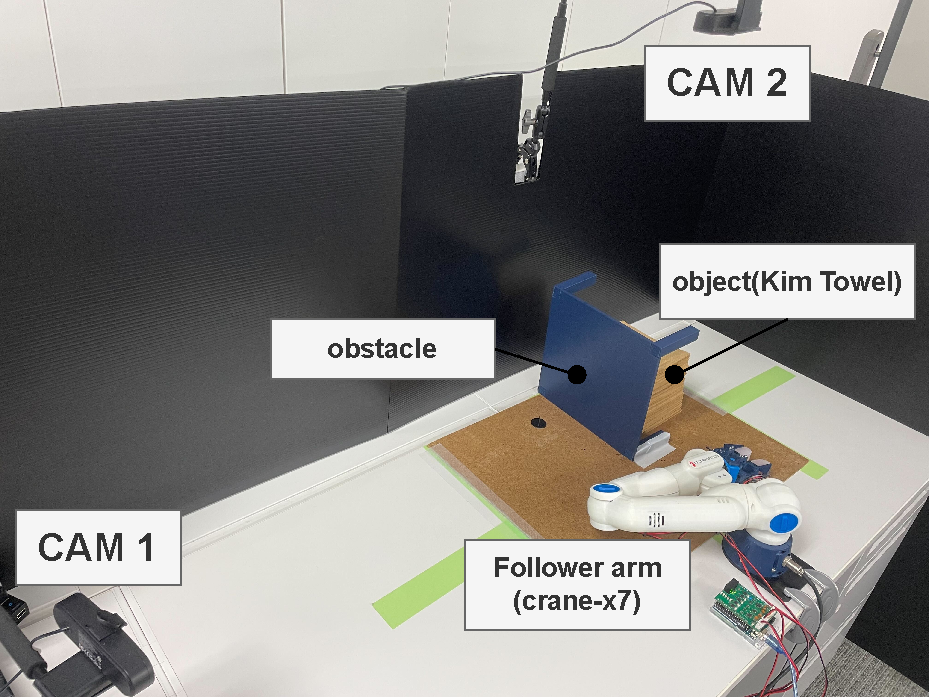
\includegraphics[width=\linewidth]{tex/Image/experimentsetup.drawio.pdf}
  \end{minipage}\hfill
  \begin{minipage}[t]{0.30\linewidth}
    \vspace{0pt}
    \centering
    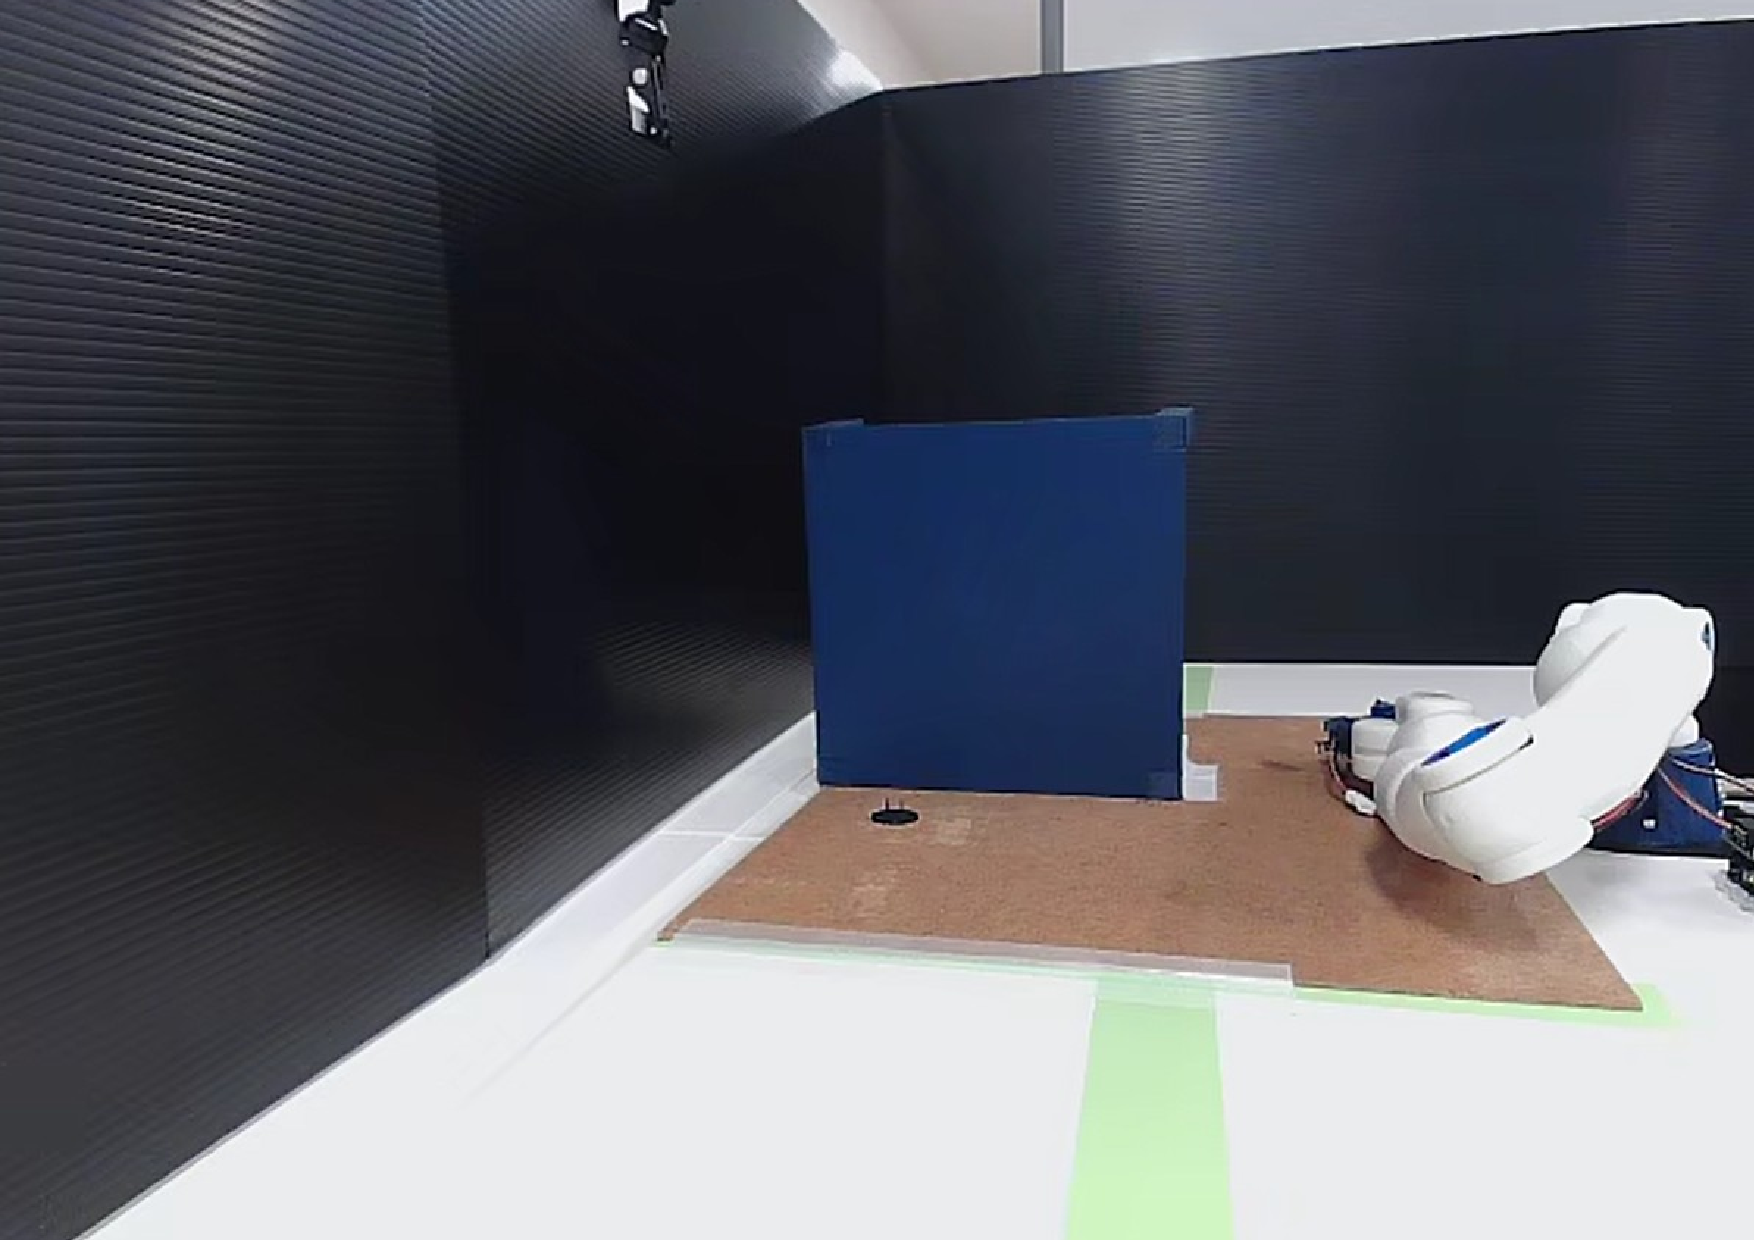
\includegraphics[width=\linewidth]{tex/Image/lateralview.pdf}
    {\footnotesize CAM1\par}
    \vspace{0.5mm}
    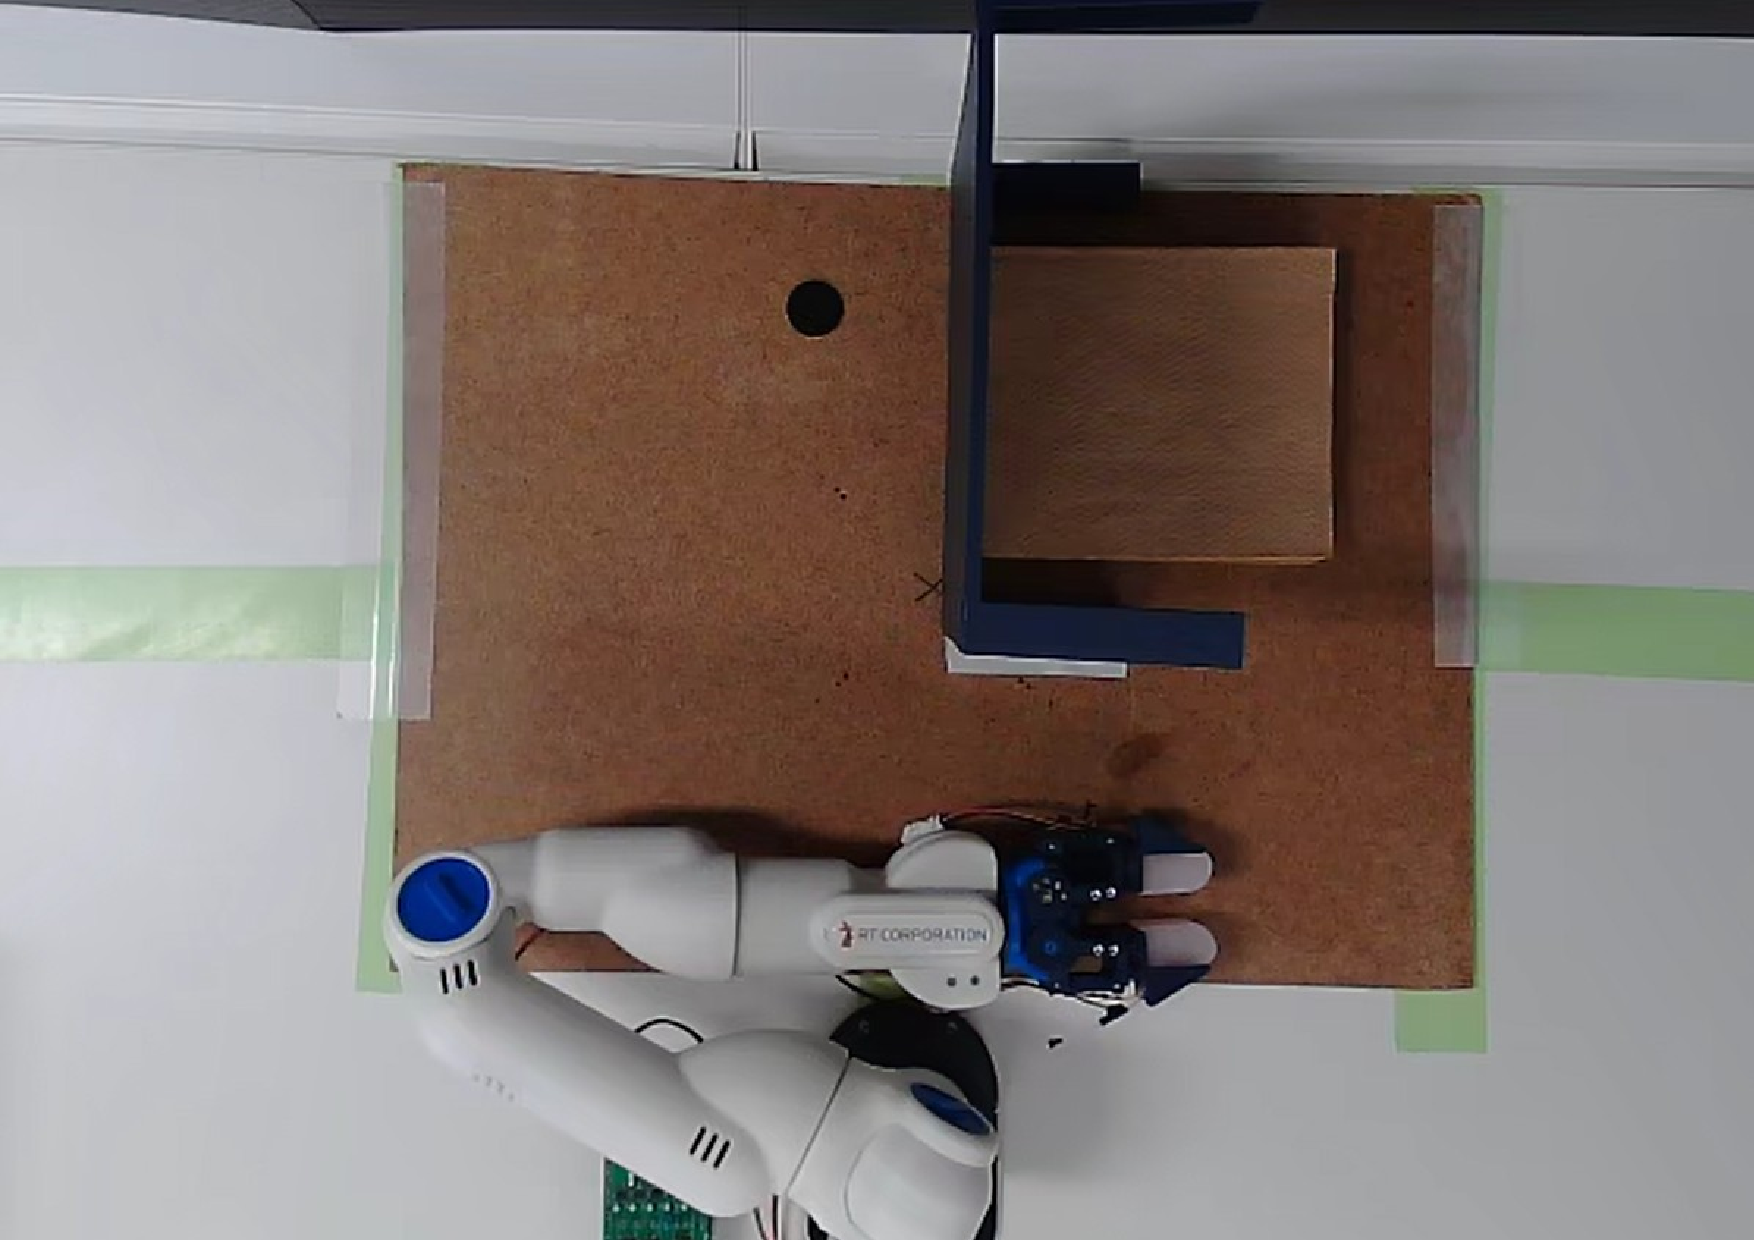
\includegraphics[width=\linewidth]{tex/Image/topview.pdf}
    {\footnotesize CAM2\par}
  \end{minipage}
  \caption{Experimental setup and camera views. The obstacle occludes the Kim towel in Camera 1 (lateral), while Camera 2 provides the top view.}
  \label{fig:experiment_setup_grasp}
\end{figure}
\vspace{-1.0ex}
本実験では，触覚情報の有用性を検証するため，触覚センサ情報の有無（sensor\_on / sensor\_off）によるタスク成功率を比較した．タスクは，積層キムタオルを把持して所定位置へ搬送する動作とした．また，双腕協調作業や深箱内操作で生じる視覚遮蔽を再現するため，Fig.~\ref{fig:experiment_setup_grasp}のように中央に障害物を設置し，側面カメラ（Camera 1）から対象物（キムタオル）の高さ情報が得られない環境を構築した．\par

教示データは，Fig.~\ref{fig:experiment_setup_grasp}のセットアップでリーダーアームをテレオペレーションし，積層キムタオルの最上位1枚を把持して障害物左側へ搬送する動作から収集した．積層枚数は50，40，30，20，10枚の5条件とし，各条件2回，計10回分を収集した．収集時には触覚センサの生データ値も記録し，学習ではセンサ値を使用しない条件（sensor\_off）と使用する条件（sensor\_on）の2条件でモデルを生成した．学習モデルのトレーニングは，AMD Ryzen 9 9950X CPU，NVIDIA GeForce RTX 5080 GPU (16GB)，メモリ64GBを搭載したPC（OS: Ubuntu 24.04.3 LTS）で実施した．ハイパーパラメータは，バッチサイズ8，学習ステップ数20,000に設定した．学習時間はいずれも約40分であった．\par

続いて，タスクの評価方法と成功率を示す．タスクの成功条件は，「積層キムタオルから1枚のみを把持し，障害物左側の目標領域へ搬送すること」と定義した．目標領域は障害物左側全域である．最初の把持動作でキムタオルを掴み損ね，ロボットが自律的に再把持（リトライ）した場合は，以降の動作にかかわらず失敗と判定した．以下に各条件での成功率を示す．教示時にはない1枚と60枚の場合を加えて，それぞれ5回の試行を行いその成功率を算出した．
% Table\ref{tab:success_rate_30mm}は指先を教示データと同じ長さにした場合，Table\ref{tab:success_rate_0mm}は指先を30mm短くした場合の成功率である．\par

\definecolor{sensoroncolor}{gray}{0.20}
\definecolor{sensoroffcolor}{gray}{0.75}

\begin{figure}[htbp]
  \centering
  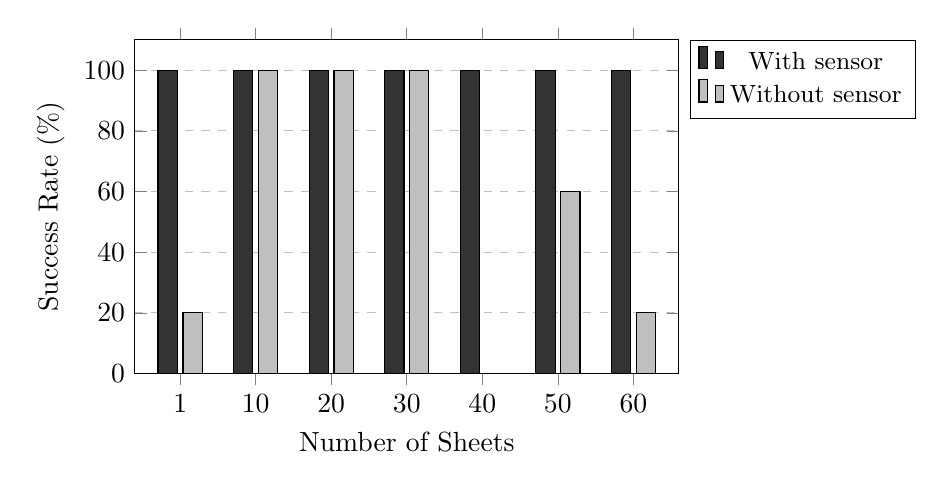
\begin{tikzpicture}
    \begin{axis}[
      ybar,
      bar width=7pt,
      xlabel={Number of Sheets},
      ylabel={Success Rate (\%)},
      xtick=data,
      symbolic x coords={1,10,20,30,40,50,60},
      ymin=0, ymax=110,
      ytick={0,20,...,100},
      ymajorgrids=true,
      grid style={dashed, gray!50},
      legend style={at={(1.02,1)}, anchor=north west, font=\small},
      width=0.70\linewidth,
      height=0.48\linewidth,
    ]
    \addplot[fill=sensoroncolor, draw=black] coordinates {
      (1,100) (10,100) (20,100) (30,100) (40,100) (50,100) (60,100)
    };
    \addlegendentry{With sensor}
    \addplot[fill=sensoroffcolor, draw=black] coordinates {
      (1,20) (10,100) (20,100) (30,100) (40,0) (50,60) (60,20)
    };
    \addlegendentry{Without sensor}
    \end{axis}
  \end{tikzpicture}
  \caption{Success rates with and without tactile sensing.}
  \label{fig:success_rate}
\end{figure}
\vspace{-1.0ex}

sensor\_on条件は教示データに含まれない高さ条件でも成功率100\%を達成した．一方，sensor\_off条件では，把持高さが教示データと異なる場合に成功率が著しく低下し，同一高さでも一部で低下が見られた．これは，ソフトフィンガー接触時の抵抗値変化をトリガーに把持動作が調整された，すなわち，触覚情報が視覚情報の不確実性を補完したと示唆される．
sensor\_off条件の失敗エピソードでは，アームが対象手前で停止する，あるいは押し込みながらつかみ損ねる動作が見られた．このことから，失敗は画像特徴量による高さ推定精度の不足に起因すると考えられる．
% また，指の長さが教示時より短い場合でも，sensor\_on条件は概ね高い成功率を維持した．ただし，対象物が1枚の場合は把持に失敗し，成功率は0\%となった．\par